%------------------------------------------%
% Cannabis Data Science
% Date: 3/9/2022
%------------------------------------------%
\documentclass[xcolor={dvipsnames}]{beamer}
\hypersetup{pdfpagemode = FullScreen}
\mode<presentation>{
  \usetheme{Boadilla}
  \usecolortheme{orchid}
  \usefonttheme{default}
  \setbeamertemplate{navigation symbols}{}
  \setbeamertemplate{caption}[numbered]
}
\setbeamersize{
  text margin left = 0.5in,
  text margin right = 0.5in
}

%------------------------------------------%
% Title
%------------------------------------------%
\title[\textbf{Cannabis Data Science \#56}]{}
\author{Cannabis Data Science}
\institute[]{\Large Cannabis Data Science \#56}
\date{March \nth{9}, 2022}

%------------------------------------------%
% Packages
%------------------------------------------%
\usepackage[english]{babel}
\usepackage[utf8x]{inputenc}
\usepackage{tikz} % For styling.
\usepackage{xparse}

%------------------------------------------%
% Colors
%------------------------------------------%
\definecolor{Green}{RGB}{34, 153, 84}
\definecolor{LightGreen}{RGB}{218, 247, 166}
\definecolor{DarkGreen}{RGB}{2, 48, 32}
\definecolor{Orange}{RGB}{255, 87, 51}
\definecolor{DarkOrange}{RGB}{199, 0, 57}
\definecolor{Yellow}{RGB}{255, 195, 0}

%------------------------------------------%
% Theme
%------------------------------------------%
\setbeamercolor*{palette primary}{bg=LightGreen, fg=DarkGreen}
\setbeamercolor*{palette secondary}{bg=LightGreen, fg=DarkGreen}
\setbeamercolor*{palette tertiary}{bg=LightGreen, fg=DarkGreen}

%------------------------------------------%
% Packages
%------------------------------------------%
\usepackage{amsmath}
\renewcommand*\footnoterule{} % No separating line on footnote.
\usepackage{mathtools} % For annotating equations.
\usepackage{hhline} % for double bars.
\usepackage[super]{nth} % For formatting 1st, 2nd, 3rd, etc.
\usepackage{graphicx, caption, subcaption}

%------------------------------------------%
% Commands
%------------------------------------------%

% Top space.
\newcommand\T{\rule{0pt}{2.5ex}}

% Bottom space.
\newcommand\B{\rule[-1.25ex]{0pt}{0pt}}

% Blocks.
\newenvironment<>{Block}[2][.9\textwidth]
  {\setlength{\textwidth}{#1}
  \begin{actionenv}#3
    \def\insertblocktitle{#2}\par
    \usebeamertemplate{block begin}}
  {\par\usebeamertemplate{block end}
  \end{actionenv}}

% Balls.
\defbeamertemplate{enumerate item}{largeball}
{\begin{pgfpicture}{-1ex}{-0.65ex}{1.5ex}{1.5ex}
\usebeamercolor[fg]{item projected}
{\pgftransformscale{2.5}\pgftext{\Large\pgfuseshading{bigsphere}}}
{\pgftransformshift{\pgfpoint{0pt}{0.5pt}}
\pgftext{\usebeamerfont*{item projected}\small\insertenumlabel}}
\end{pgfpicture}}

% Fancy arrows.
\NewDocumentCommand\UpArrow{O{2.0ex} O{black}}{%
   \mathrel{\tikz[baseline] \draw [->, line width=0.5pt, #2] (0,0) -- ++(0,#1);}} % Fancy up-arrow.
\NewDocumentCommand\DownArrow{O{2.0ex} O{black}}{%
   \mathrel{\tikz[baseline] \draw [<-, line width=0.5pt, #2] (0,0) -- ++(0,#1);}} % Fancy down-arrow.

% Equations with numbers on the left.
\makeatletter
\newcommand{\LeftEqNo}{\let\veqno\@@leqno}
\makeatother

%------------------------------------------%
% Presentation
%------------------------------------------%
\begin{document}

% Title page.
\begin{frame}{}
  
\includegraphics[scale=0.33]{images/logo.pdf}
  \vspace*{-2\baselineskip}
  \titlepage

  % TODO: Add flare to title page?
  % Background
%\tikz[remember picture, overlay]
%\node[opacity=1.0, inner sep=0pt] at (current page.center){
%  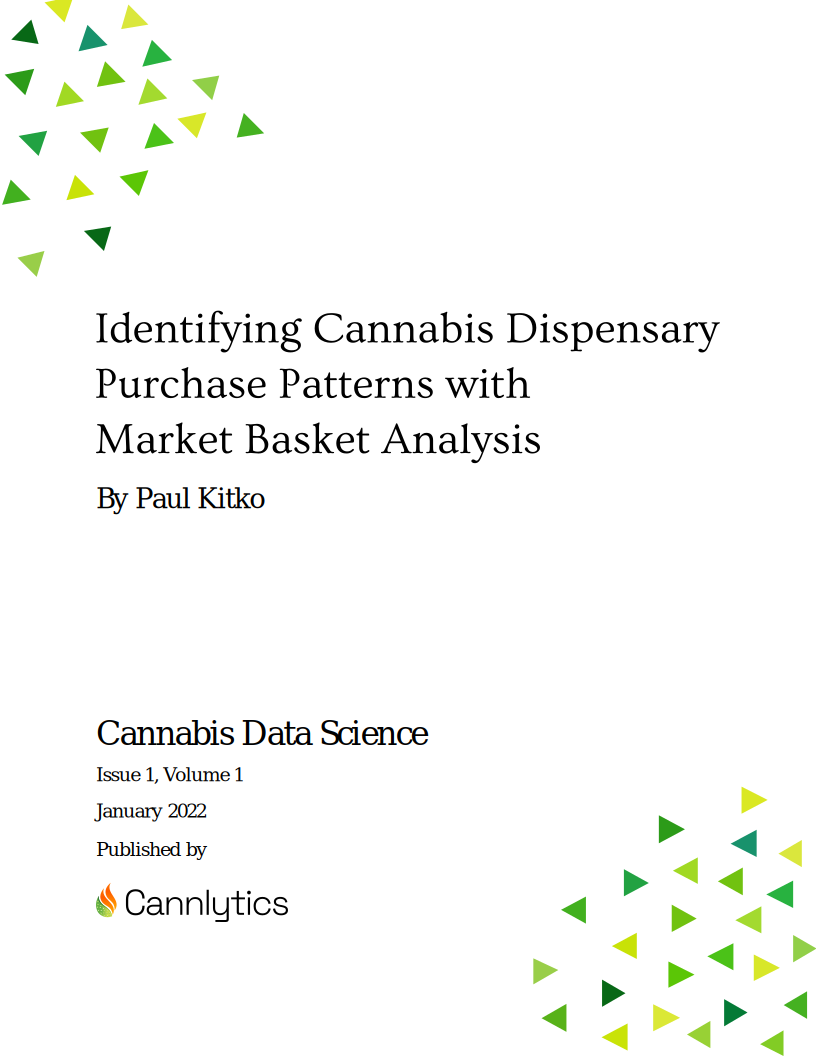
\includegraphics[width=\paperwidth, height=\paperheight]{images/cover.pdf}
%};  
  
\end{frame}

%------------------------------------------%
% Introduction
%------------------------------------------%
\section{Introduction}

\begin{frame}{}

\begin{minipage}{0.7\textwidth}

\vspace{-2\baselineskip}

% Question of the day
\begin{center}
\begin{minipage}{.9\linewidth}
\begin{Block}{Yield is the name of the game.}

\vspace{.5\baselineskip}
\begin{itemize}
\item  Does the amount a producer produces affect the \underline{number of periods} a producer has operated or if a producer has \underline{exited}?

\vspace{.5\baselineskip}

\item Does the amount a retailer sells affect the \underline{number of periods} that they have operated or if they have \underline{exited}?
\end{itemize}

\vspace{.5\baselineskip}

\end{Block}
\end{minipage}
\end{center}

\end{minipage}\hspace{0.05\textwidth}%
\begin{minipage}{0.25\textwidth}

\vspace{0.5\baselineskip}

\begin{figure}
\includegraphics[height=2.in]{images/free-entry.jpg}
\caption*{%
  \tiny
  {Free entry sign in Germany.\\Author: Lupus in Saxonia\\ License: CC-BY-SA 4.0 https://creativecommons.org/licenses/by-sa/4.0/deed.en}
 }
\end{figure}

\end{minipage}

% Free entry sign in Germany.
% Author: Lupus in Saxonia
% License: CC-BY-SA 4.0 https://creativecommons.org/licenses/by-sa/4.0/deed.en

\end{frame}

%------------------------------------------%
% Survival Analysis
%------------------------------------------%

\begin{frame}{}

{\large \textbf{Survival Analysis}}\vspace{0.5\baselineskip}\\

\begin{itemize}

\item {\bfseries Survival analysis} is a branch of statistics for analyzing the \underline{expected duration} of time until \underline{one event occurs}.

\vspace{\baselineskip}

\item Can fit a parametric {\bfseries survival function}

$$S(t \hspace{0.5ex}\vert\hspace{0.5ex} \beta, X) = P(T>t \hspace{0.5ex}\vert\hspace{0.5ex} \beta, X)$$

%\vspace{\baselineskip}

%\item Can handle {\bfseries censored data} -- data where the event of interest has not occurred.

\end{itemize}

\vspace{0.5\baselineskip}

\begin{figure}
\includegraphics[height=1.5in]{images/treatment-survival-function.png}
\caption*{%
  \tiny
  {Survival function for treated and untreated leukemia.\\Author: Michaelg2015\\ License: CC-BY-SA 4.0 https://creativecommons.org/licenses/by-sa/4.0/deed.en}
 }
\end{figure}

\end{frame}


%------------------------------------------%
% Consumption Rates
%------------------------------------------%

%\begin{frame}{}
%
%{\large \textbf{Consumption Rates}}\vspace{\baselineskip}\\
%
%\end{frame}


%------------------------------------------%
% Natural Language Processing
%------------------------------------------%

\begin{frame}{}

{\large \textbf{Natural Language Processing}}\vspace{\baselineskip}\\

\begin{minipage}{0.8\textwidth}

\begin{itemize}

\item {\bfseries Symbolic methods} -- hand--coding a set of rules to be used with dictionary lookup.

%\vspace{0.5\baselineskip}
%
%\begin{itemize}
%
%\item Pros:
%
%\vspace{0.5\baselineskip}
%
%\item Cons:
%
%\end{itemize}

\vspace{0.5\baselineskip}

\item {\bfseries Machine-learning algorithms} -- systems based on automatically learning rules can be made more accurate simply by supplying more input data.

%\vspace{0.5\baselineskip}
%
%\begin{itemize}
%
%\item Pros:
%
%\vspace{0.5\baselineskip}
%
%\item Cons:
%
%\end{itemize}
%
\end{itemize}

\end{minipage}\hspace{0.05\textwidth}%
\begin{minipage}{0.15\textwidth}

\begin{figure}
\includegraphics[height=1in]{images/parse-tree.png}
\end{figure}

\end{minipage}


\end{frame}

%------------------------------------------%
% Natural Language Processing with SpaCy
%------------------------------------------%

%Semantic role labelling


% Named entity recognition

%Relationship extraction

%\begin{frame}{}
%
%{\large \textbf{Natural Language Processing with SpaCy}}\vspace{\baselineskip}\\
%
%\begin{itemize}
%
%\item {\bfseries EntityRecognizer} -- This component is referred as ner. It is responsible for identifying named entities and assigning labels to them.
%
%\item {\bfseries EntityRuler} -- This component is called * entity_ruler*.It is responsible for assigning named entitile based on pattern rules. Revisit Rule Based Matching to know more.
%
%\end{itemize}
%
%\end{frame}

%Tokenizer : It is responsible for segmenting the text into tokens are turning a Doc object. This the first and compulsory step in a pipeline.
%Tagger : It is responsible for assigning Part-of-speech tags. It takes a Doc as input and createsDoc[i].tag
%DependencyParser : It is known as parser. It is responsible for assigning the dependency tags to each token. It takes a Doc as input and returns the processed Doc
%EntityRecognizer : This component is referred as ner. It is responsible for identifying named entities and assigning labels to them.
%TextCategorizer : This component is called textcat. It will assign categories to Docs.
%EntityRuler : This component is called * entity_ruler*.It is responsible for assigning named entitile based on pattern rules. Revisit Rule Based Matching to know more.
%Sentencizer : This component is called **sentencizer** and can perform rule based sentence segmentation.
%merge_noun_chunks : It is called mergenounchunks. This component is responsible for merging all noun chunks into a single token. It has to be add in the pipeline after tagger and parser.
%merge_entities : It is called merge_entities .This component can merge all entities into a single token. It has to added after the ner.
%merge_subtokens : It is called merge_subtokens. This component can merge the subtokens into a single token.



%------------------------------------------%
% Takeaway
%------------------------------------------%
\section{Takeaway}
\begin{frame}{}

\begin{center}
\begin{minipage}{3.85in}

% Thank you.
\includegraphics[width=.25in]{images/prayer.png} {\Large \textbf{Thank you for coming.}}\\

\begin{center}
\begin{minipage}{.9\linewidth}
\begin{Block}{Lesson of the Day}

\vspace{0.5\baselineskip}

\begin{itemize}

\item Parsing natural language can be complex, but can yield valuable data.

\vspace{0.5\baselineskip}

\end{itemize}

\end{Block}
\end{minipage}
\end{center}

\vfill

\end{minipage}
\end{center}

\end{frame}

%------------------------------------------%
% Fin.
%------------------------------------------%
\end{document}
